Eine der besten Möglichkeiten, Temperaturen zu messen, ist die Infrarottechnik.
Sie bietet einige erhebliche Vorteile, durch die Fähigkeit zur berührungslosen
Temperaturmessung. Zum einen wird der zu messende Gegenstand in keinerlei Weise
beeinflusst, was zum Beispiel die Gefahr der physischem Zerstörung, durch
Berühren empfindlicher Gegenstände, wie Blätter verhindert. (Abb 4.1) Die
Entfernung zum Messpunkt ermöglicht auch, sehr hohe Temperaturen zu messen,
ohne die Infrarotsensorik durch zu hohe Temperaturen zu gefährden.

\begin{figure}[ht]
    \centering
    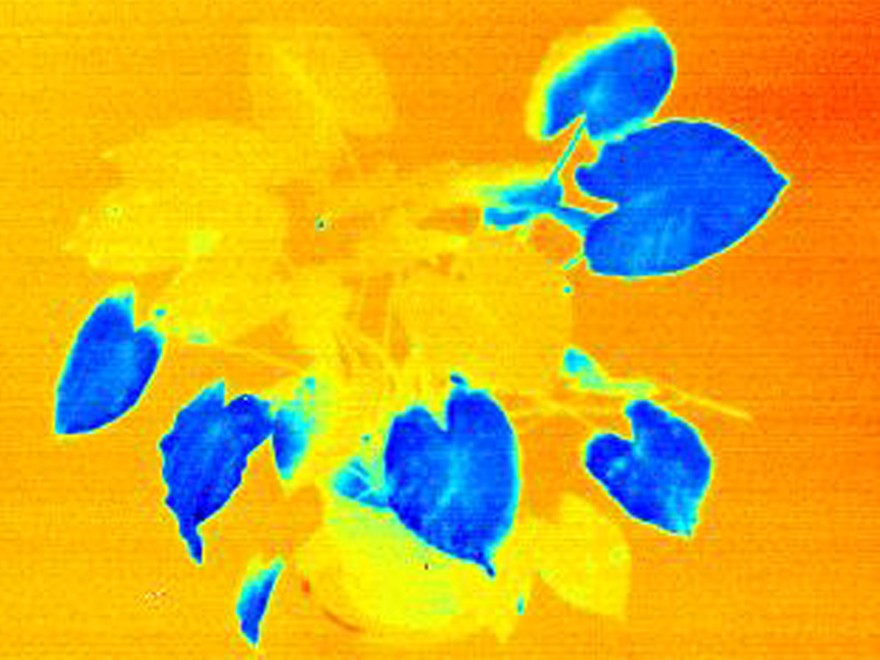
\includegraphics[width=0.5\textwidth]{bilder/infrarot_pflanze.jpg}
    \caption[Infrarotaufnahme einer Pflanze]{Infrarotaufnahme einer Pflanze}
    \label{fig:Infrarotaufnahme Pflanze}
\end{figure}

Funktionsweise von Infrarotthermographie: \\
Messgegenstände mit einer Temperatur von > 900K strahlen Energie ab, der in mithilfe von Wärmebildtechnik sichtbar gemacht werden kann und so als Bild, für den Menschen sichtbar dargestellt werden kann.
Hierzu werden die Spektralbereiche Nahinfrarot(NIR), mittleres Infrarot (MIR) und langes Infrarot (LIR) betrachtet. 
Diese Spektren teilen sich in drei Teile im Bereich von 780 bis 14000nm auf. \cite{schuster2004infrarotthermographie}
